\documentclass[10pt,twoside,a4paper, twocolumn]{article}

%  EDIT THIS SECTION  %%%%%%%%%%%%%%%%%%%%%%%%%%%%%%%%%%%%%%%%%%%%%%%%%%%%%%%%%%%%%
\newcommand{\Title}{\sc A \LaTeX \ template for Volcanica} % Manuscript title goes here
\newcommand{\Author}{Nafn et al.\xspace} % First author goes here. Leave blank if opting for blind review.
\newcommand{\Year}{2017} % Year goes here
%%%%%%%%%%%%%%%%%%%%%%%%%%%%%%%%%%%%%%%%%%%%%%%%%%%%%%%%%%%%%%%%%%%%%%%%%%


%  DO NOT EDIT THIS SECTION  %%%%%%%%%%%%%%%%%%%%%%%%%%%%%%%%%%%%%%%%%%%%%%%%%%%%%%%%
\pdftrailerid{} %Remove ID
\pdfsuppressptexinfo15 %Suppress PTEX.Fullbanner and info of imported PDFs

\usepackage[affil-sl]{authblk}
\setcounter{Maxaffil}{3}
\renewcommand\Affilfont{\itshape\small}
\renewcommand{\thefootnote}{\fnsymbol{footnote}}

\usepackage{titlesec}
\titleformat*{\section}{\large \sc \bfseries}
\titleformat*{\subsection}{}
\titleformat*{\subsubsection}{\sl}
\renewcommand{\thesubsubsection}{\emph{\thesubsection.\arabic{subsubsection}}}

\usepackage{xcolor}
\definecolor{maroon}{rgb}{0.5, 0.0, 0.0}
\definecolor{PUSblue}{HTML}{005FA8}
\usepackage{hyperref} \hypersetup{colorlinks = true, citecolor = PUSblue}

\usepackage{lipsum}
\usepackage{fancyhdr}
\usepackage[french,english]{babel}

\usepackage[utf8]{inputenc} 
\usepackage[]{kpfonts}
\usepackage[T1]{fontenc}

\usepackage{graphicx}
\usepackage{booktabs}
\usepackage{longtable}
\usepackage{siunitx}
\usepackage[sectionbib,square,elide]{natbib}
\bibliographystyle{apalike}

\usepackage{draftwatermark}
\SetWatermarkText{\sc DRAFT}
\SetWatermarkScale{1}
\SetWatermarkColor[gray]{0.85}

\usepackage{lineno}
\linenumbers % Enable line numbers to facilitate review process. 

\usepackage[tmargin=1in,bmargin=1in,lmargin=0.9 in,rmargin=0.9in]{geometry} 

\usepackage{abstract}
\renewcommand{\abstractnamefont}{\normalfont \large \sc \bfseries}

\pagestyle{fancy}
\fancyhf{}
\fancyhead[LE]{\Title}
\fancyhead[RE]{\sc \Author, \ \Year}
\rfoot{Page \thepage}
\lfoot{
\includegraphics[width=\columnwidth]{PUSbanner}}
\fancypagestyle{firststyle}
{
   \fancyhf{}
   \fancyhead{
\includegraphics[width=\textwidth]{article_banner}}
}
\title{\Title}
%%%%%%%%%%%%%%%%%%%%%%%%%%%%%%%%%%%%%%%%%%%%%%%%%%%%%%%%%%%%%%%%%%%%%%%%%%

%  EDIT THIS SECTION  %%%%%%%%%%%%%%%%%%%%%%%%%%%%%%%%%%%%%%%%%%%%%%%%%%%%%%%%%%%%%
\author{%
Falsa Nafn\thanks{Affiliation 1}\thanks{Corresponding author: {\texttt{myemail@somewhere.world}}}, N. Ambardo\thanks{Affiliation 2}, and Una Terza\thanks{Affiliation 3}%
} % Author list goes here, with affiliations defined using \thanks{}. Corresponding author email address is defined in the same way. Leave blank if opting for blind review.
%%%%%%%%%%%%%%%%%%%%%%%%%%%%%%%%%%%%%%%%%%%%%%%%%%%%%%%%%%%%%%%%%%%%%%%%%%

%  DO NOT EDIT THIS SECTION  %%%%%%%%%%%%%%%%%%%%%%%%%%%%%%%%%%%%%%%%%%%%%%%%%%%%%%%%
\begin{document}
\date{}
\twocolumn[
  \begin{@twocolumnfalse}
    \maketitle
\thispagestyle{firststyle}
%%%%%%%%%%%%%%%%%%%%%%%%%%%%%%%%%%%%%%%%%%%%%%%%%%%%%%%%%%%%%%%%%%%%%%%%%%

%  EDIT THIS SECTION  %%%%%%%%%%%%%%%%%%%%%%%%%%%%%%%%%%%%%%%%%%%%%%%%%%%%%%%%%%%%%
\selectlanguage{english}
\begin{abstract}
Abstract text goes here. \textbf{No more than 150 words}. Lorem ipsum dolor sit amet, consectetur adipiscing elit. Integer nec odio. Praesent libero. Sed cursus ante dapibus diam. Sed nisi. Nulla quis sem at nibh elementum imperdiet. Duis sagittis ipsum. Praesent mauris. Fusce nec tellus sed augue semper porta. Mauris massa. Vestibulum lacinia arcu eget nulla. Class aptent taciti sociosqu ad litora torquent per conubia nostra, per inceptos himenaeos. Curabitur sodales ligula in libero. Sed dignissim lacinia nunc. Curabitur tortor. Pellentesque nibh. Aenean quam. In scelerisque sem at dolor. Maecenas mattis. Sed convallis tristique sem. Proin ut ligula vel nunc egestas porttitor. Morbi lectus risus, iaculis vel, suscipit quis, luctu.
\end{abstract}
\selectlanguage{french}
\begin{abstract}
A second-language abstract can go here. \textbf{No more than 150 words}. Lorem ipsum dolor sit amet, consectetur adipiscing elit. Integer nec odio. Praesent libero. Sed cursus ante dapibus diam. Sed nisi. Nulla quis sem at nibh elementum imperdiet. Duis sagittis ipsum. Praesent mauris. Fusce nec tellus sed augue semper porta. Mauris massa. Vestibulum lacinia arcu eget nulla. Class aptent taciti sociosqu ad litora torquent per conubia nostra, per inceptos himenaeos. Curabitur sodales ligula in libero. Sed dignissim lacinia nunc. Curabitur tortor. Pellentesque nibh. Aenean quam. In scelerisque sem at dolor. Maecenas mattis. Sed convallis tristique sem. Proin ut ligula vel nunc egestas porttitor. Morbi lectus risus, iaculis vel, suscipit quis, luctu.
\end{abstract}
\vspace{5mm}
\vspace{5mm}
  \end{@twocolumnfalse}
]
\saythanks
\section{Introduction}

\subsection{Subsections appear like this}
\subsubsection{And  sub-subsections appear like this}

Equations are defined in the \{equation\} environment:
 \begin{equation}
\frac{n!}{k!(n-k)!} = \binom{n}{k}
\end{equation}

\begin{equation}
\lim_{x \to \infty} \exp(-x) = 0
\end{equation}

Citations may either be inline: \citet{einstein1935particle} or in parentheses \citep{einstein1935particle}.

The main body of the text should go here, with footnotes\footnote{such as this one} used when appropriate.
\section{Lipsum}
\lipsum

\begin{figure}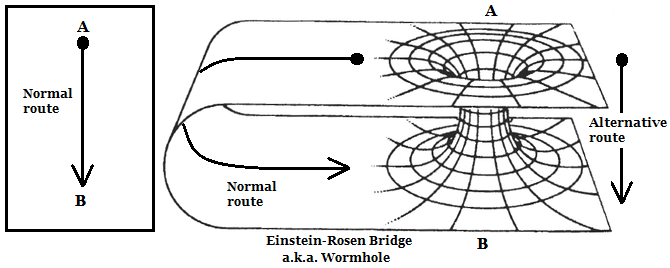
\includegraphics[width=\columnwidth]{ER-bridge} 
\caption{Einstein--Rosen bridge (``wormhole'').}
\label{fig:1}
\end{figure}
\section{More Lipsum}

\lipsum

\section*{Acknowledgements} % Please upload separately if opting for blind review.
Thank all relevant parties and acknowledge funding sources, if any.
\section*{Author contributions} % Please upload separately if opting for blind review.
Tell us who did what.
\section*{Data availability}
Authors should direct readers to an open access repository such as figshare or Github, where data are made available.
\bibliography{mybibfile} % a separate bibfile is required. Please upload this file along with the compiled manuscript and source file.

%%%%%%%%%%%%%%%%%%%%%%%%%%%%%%%%%%%%%%%%%%%%%%%%%%%%%%%%%%%%%%%%%%%%%%%%%%
\end{document}
